%
% File acl2014.tex
%
% Contact: koller@ling.uni-potsdam.de, yusuke@nii.ac.jp
%%
%% Based on the style files for ACL-2013, which were, in turn,
%% Based on the style files for ACL-2012, which were, in turn,
%% based on the style files for ACL-2011, which were, in turn, 
%% based on the style files for ACL-2010, which were, in turn, 
%% based on the style files for ACL-IJCNLP-2009, which were, in turn,
%% based on the style files for EACL-2009 and IJCNLP-2008...

%% Based on the style files for EACL 2006 by 
%%e.agirre@ehu.es or Sergi.Balari@uab.es
%% and that of ACL 08 by Joakim Nivre and Noah Smith

\documentclass[11pt]{article}
\usepackage{acl2014}
\usepackage{times}
\usepackage{url}
\usepackage{latexsym}


%%%%%% ADDED TO GET CORRECT PDF SIZE
\pdfpagewidth=\paperwidth
\pdfpageheight=\paperheight


%%%%%% EXTRA PACKAGES
\usepackage{graphicx}
\usepackage{listings}
\usepackage{tabularx}
\usepackage{ctable}
\usepackage{booktabs}
\usepackage{multirow}
\usepackage{rotating}


%\setlength\titlebox{5cm}

% You can expand the titlebox if you need extra space
% to show all the authors. Please do not make the titlebox
% smaller than 5cm (the original size); we will check this
% in the camera-ready version and ask you to change it back.


\title{\textit{lex4all}: A language-independent tool for building and evaluating pronunciation lexicons for small-vocabulary speech recognition}

%\author{Anjana Vakil \\
%  Affiliation / Address line 1 \\
%  Affiliation / Address line 2 \\
%  Affiliation / Address line 3 \\
%  {\tt email@domain} \\\And
%  Max Paulus \\
%  Affiliation / Address line 1 \\
%  Affiliation / Address line 2 \\
%  Affiliation / Address line 3 \\
%  {\tt email@domain} \\}

\date{}

\begin{document}
\maketitle

\begin{abstract}
This paper describes \textit{lex4all}, an open-source PC application for the generation and evaluation of pronunciation lexicons in any language. 
With just a few minutes of recorded audio and no expert knowledge of linguistics or speech technology, individuals or organizations seeking to create speech-driven applications in low-resource languages can use this tool to build  lexicons enabling 
the recognition of small vocabularies (up to 100 words, roughly) in the target language
%small-vocabulary speech recognition in the target language 
using an existing recognition engine designed for a high-resource source language (e.g. English). 
To build such lexicons, we employ an existing technique for cross-language phoneme-mapping; 
we describe this method and how it is implemented in \textit{lex4all}.
%we give an overview of this method and describe its implementation in \textit{lex4all}. 
%Beyond the core functionality of building new lexicons, the tool also offers 
The application also offers
a built-in audio recorder that facilitates data collection, 
a significantly faster implementation of the phoneme-mapping algorithm,
and an evaluation module that expedites research on small-vocabulary speech recognition for low-resource languages. 
%Finally, we report on an investigation into the impact of varying the high-resource source language used; our results seem to indicate that phonetic similarity between target and source language does not significantly affect recognition accuracy, underscoring the system's language-independence.
\end{abstract}


%Demo submissions should also clearly indicate if any computer equipment is expected to be provided by the local organizer. If so, please specify desired hardware platform, hard disk and memory capacity, operating system and other software needed in order to run the demo. 
%
%Implementation of ACL multiple submission policy: Papers being submitted both to ACL and another conference or workshop must
%\begin{itemize}
%\item Note on the title page the other conference or workshop to which they are being submitted. (This includes submissions that are extensions of papers currently being submitted to a workshop.)
%\item State on the title page that if the paper is accepted for ACL, then the paper will be withdrawn from other conferences and workshops.
%\end{itemize}
%Papers that overlap other papers that have appeared at a conference with published proceedings must contain significant new results. Authors must include on the title page a list of any previous papers that the current paper overlaps or extends, and must identify the significant new results contained in the new submission. The program co-chairs have the final decision about what constitutes significant new results.

\section{Introduction\footnote{Parts of this paper (Sections \ref{sec:intro} and \ref{sec:background}) overlap with a paper submitted to the 4th Workshop on Spoken Language Technologies for Under-resourced languages (SLTU '14, http://www.mica.edu.vn/sltu2014). That paper, which is currently under review, concerns related research not reported here, and makes no mention of the \textit{lex4all} application.}}
\label{sec:intro}

In recent years it has been demonstrated that speech recognition interfaces can be extremely beneficial for applications in the developing world
%, particularly in communities where literacy rates are low 
%or where PCs and internet connections are not always available
 \cite{case4st4d,Sherwani09,bali13}. 
Typically, 
such applications target low-resource languages (LRLs) for which large collections of speech data are unavailable, preventing the training or adaptation of recognition engines for these languages.
%the languages spoken in such communities are under-resourced, such that the large audio corpora typically needed to train or adapt recognition engines are unavailable.
%, and collecting such vast amounts of data is generally infeasible for individuals or small organizations interested in developing speech-driven applications for their communities. 
However, 
%in the absence of a recognition engine trained for the target low-resource language (LRL), 
an existing recognizer for a completely unrelated high-resource language (HRL), such as English, can be used to perform small-vocabulary recognition tasks in the LRL,
%(By ``small-vocabulary tasks'' we mean those requiring discrimination between a few dozen terms.) 
%of the type required in grammar-controlled applications (e.g. for accessing information or conducting basic transactions), which may require the system to distinguish a few dozen terms in the URL. 
provided a pronunciation lexicon mapping each term in the target vocabulary to a sequence of phonemes in the HRL, i.e. phonemes which the recognizer can model. 

This is the motivation behind \textit{lex4all},\footnote{http://lex4all.github.io/lex4all/} an open-source application that allows users to automatically create a mapped pronunciation lexicon for terms in any language, using a small number of speech recordings and an out-of-the-box recognition engine for a HRL. The resulting lexicon can then be used with the HRL recognizer to add small-vocabulary speech recognition functionality to applications in the LRL, without the need for the large amounts of data and expertise in speech technologies required to train a new recognizer. This paper describes the \textit{lex4all} application and its utility for the rapid
%, simple 
creation and evaluation of pronunciation lexicons enabling small-vocabulary speech recognition in any language.

\section{Background and related work}
\label{sec:background}
Several commercial speech recognition systems offer high-level Application Programming Interfaces (APIs) that 
make it extremely simple to add voice interfaces to an application, requiring
%make adding voice recognition capabilities to an application 
%as simple as specifying (in text) the words/phrases that should be recognized; this requires 
very little general technical expertise and virtually no knowledge of the inner workings of the recognition engine. If the target language is supported by the system -- the Microsoft Speech Platform, for example, supports 
%recognition and synthesis for 
over 20 languages \cite{mspsdk} -- this makes it very easy 
%for small-scale software developers (i.e. individuals or small organizations with limited funding) 
to create speech-driven applications. 

If, however, the target language is one of the many thousands of LRLs for which high-quality recognition engines have not yet been developed, alternative strategies for developing speech-recognition interfaces must be employed.
%While many such individuals or organizations in the developing world may be interested in using such platforms to build applications for use in their communities, the LRLs typically spoken in these areas are obviously not supported by such commercial systems. 
Though tools for quickly training or adapting recognizers for new languages exist (e.g. CMUSphinx\footnote{http://www.cmusphinx.org} or the Rapid Language Adaptation Toolkit\footnote{http://i19pc5.ira.uka.de/rlat-dev}), these typically require hours of training audio to produce effective models, 
data which is by definition not available for a LRL.
Furthermore, non-expert users may struggle to effectively utilize such tools, which still demand some understanding of speech/language technologies.

However, many useful %development-oriented 
applications (e.g. for accessing information or conducting basic transactions) only require small-vocabulary recognition, i.e. discrimination between
a few dozen terms (words or short phrases).
For example, VideoKheti \cite{bali13}, a smartphone application that delivers agricultural information to farmers in India using a Hindi speech interface, uses a vocabulary of 79 terms.
For such small-vocabulary applications, 
%an unmodified HRL recognizer 
an engine designed to recognize speech in a HRL
can be used as-is to perform recognition of the LRL terms,
%as Figure~\ref{fig:background} illustrates, 
%we simply provide the recognizer with 
given
a grammar describing the allowable combinations/sequences of terms to be recognized, and a pronunciation lexicon mapping each target term to a sequence of phonemes in the HRL 
(see Figure~\ref{fig:lexicon} for an example).

%\begin{figure}[tb]
%\begin{center}
%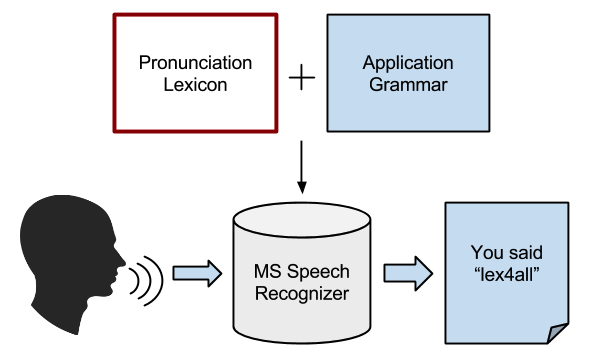
\includegraphics[width=\columnwidth]{../img/background-diagram-cropped.png}
%\caption{Given a pronunciation lexicon and application-specific grammar, an existing recognizer for a HRL can be used to recognize speech in a LRL.\label{fig:background}}
%\end{center}
%\end{figure}

%TODO syntax highlighting?
\lstset{
	%language=xml,
	basicstyle={\footnotesize\ttfamily},
	%frame=tblr,
	numbers=none,
	linewidth=\columnwidth,
	breaklines=true,
	captionpos=b,
	}
\begin{figure}
%<?xml version="1.0" encoding="utf-8"?>
\begin{lstlisting}	
<lexicon version="1.0" xmlns="http://www.w3.org/2005/01/pronunciation-lexicon" xml:lang="en-US"  alphabet="x-microsoft-ups">
		 
  <lexeme>
    <grapheme>beeni</grapheme>
    <phoneme>B E NG I</phoneme>
    <phoneme>B EI N I I</phoneme>
  </lexeme>
  
</lexicon>
\end{lstlisting}
\caption{Sample XML lexicon mapping the Yoruba word \textit{beeni} (``yes'') to two possible sequences of American English phonemes.\label{fig:lexicon}}
\end{figure}



This is the thinking behind Speech-based Automated Learning of Accent and Articulation Mapping, or ``Salaam'' \cite{Sherwani09,Qiao10,Chan12}, a
%. This 
method of cross-language phoneme-mapping 
that
%automatically 
discovers accurate source-language pronunciations for terms in the 
%(unrelated) 
target language. 
%thus constitutes the foundation on which the \textit{lex4all} tool is built.
%The Salaam method is at the core of the \textit{lex4all} lexicon-building tool.
%In the Salaam approach, an iterative algorithm uses a specially-designed recognition grammar to discover the best pronunciation(s) for a word one phoneme at a time
The basic idea 
%of phoneme-mapping 
is to discover the best pronunciation (phoneme sequence) for a target term by using the source-language recognition engine to perform phone decoding on one or more utterances of the term. As commercial recognizers such as Microsoft's are designed for word-decoding, and their APIs do not usually allow users access to the phone-decoding mode, the Salaam approach uses a specially designed  ``super-wildcard'' recognition grammar 
to mimic phone decoding 
and guide pronunciation discovery \cite{Qiao10,Chan12}.
%(Qiao~et~al., 2010, Sec.~4.1; Chan~and~Rosenfeld, 2012, Sec.~3.2).
%Specifically, Qiao et al. \cite[Sec.~4.1]{Qiao10} create a recognition grammar representing a phoneme ``super-wildcard'' that guides pronunciation discovery. 
This grammar allows the engine to recognize each sample of the target term as a ``phrase'' made up of 0-10 ``words'',
where each ``word'' can be matched to any possible sequence of 1, 2, or 3 source-language phonemes.
%\cite[Sec.~4.1]{Qiao10}. 
This allows the recognizer to identify the phoneme sequence best matching a given term, without any prior indication of how many phonemes that sequence should contain.

Given this grammar and one or more audio recordings of the target term, 
\newcite
%[Sec.~4.1]
{Qiao10} 
use an iterative training algorithm to discover the best pronunciation(s) for that term, one phoneme at a time. 
%In the first pass, the recognizer determines the best candidate(s) for the first phoneme of the term, and prefixes the phoneme(s) to the super-wildcard grammar
Essentially, the recognizer makes one pass to find the best candidate(s) for the first phoneme, then a second pass to find the first two phonemes, and so on until a stopping criterion is met, e.g. the recognition confidence score 
%assigned to the resulting ``phrase'' 
stops improving, % \cite[p.~4]{Qiao10}, 
indicating that the sequence is complete.

Compared to pronunciations hand-written by a linguist, pronunciations generated automatically by this algorithm yield substantially higher recognition accuracy: % \cite[Sec.~5.2]{Qiao10}: 
\newcite{Qiao10} report word recognition accuracy rates in the range of 75-95\% for vocabularies of 50 terms.
%Qiao et al. further improve accuracy by training on samples from multiple speakers, and by creating a lexicon with multiple pronunciations for each word (i.e. the $n$-best results of the training algorithm instead of the single best result).
%, Qiao et al. are able to further improve accuracy. 
\newcite{Chan12} improve accuracy on larger vocabularies (up to approximately 88\% for 100 terms) by applying an iterative discriminative training algorithm, identifying and removing pronunciations that cause confusion between word types.

%In sum, 
The Salaam method is fully automatic, demanding expertise neither in speech technology 
%(to modify acoustic models) 
nor in linguistics,
%(to manually generate seed pronunciations), 
%and for each new target language it requires 
and requires only a few recorded utterances of each word,
%from one or more speakers, 
an amount of data that can be collected quickly with little effort or expense. 
Despite these humble requirements, it 
%enables the construction of pronunciation lexicons that 
can help create speech-driven applications in LRLs, as has been demonstrated in at least two projects that have successfully used the Salaam method to add voice interfaces to real applications: an Urdu telephone-based health information system \cite{Sherwani09}, and
the VideoKheti application mentioned above \cite{bali13}.
What has not existed before now is an interface to make this approach accessible to any user.

Given the established success of the Salaam method 
%for pronunciation discovery, 
our contribution is to create a more time-efficient implementation of the pronunciation-discovery algorithm and integrate it into an easy-to-use graphical application, so that non-expert users can quickly and easily create lexicons to develop speech interfaces in LRLs using existing HRL recognizers. In the following sections, we describe the \textit{lex4all} application and our slightly-modified implementation of the Salaam method.

%\vfill

\section{System overview}
\label{sec:overview}

We have developed \textit{lex4all} as a desktop application for Microsoft Windows,\footnote{Windows 7 or 8 (64-bit).} since it relies on the Microsoft Speech Platform \cite{mspsdk} as explained below.
%for speech recognition (see Section~\ref{sec:engine}).
The application and its source code are freely available 
%for download 
via GitHub.\footnote{[GitHub repository link removed to preserve anonymity]} 

%As stated above, the primary functionality of \textit{lex4all} is the fast and easy construction of pronunciation lexicons; Figure~\ref{fig:system} illustrates the architecture of the lexicon-building system.
%, explained below. In addition to this core system, \textit{lex4all} also features an evaluation module that simulates recognition using a given lexicon and can be used as a research tool; this module is explained in detail in Section~\ref{sec:evaluation}.

The application's core feature is its lexicon-building tool, the architecture of which is illustrated in Figure~\ref{fig:system}.
A simple graphical user interface (GUI) allows the user to type in the written form of each term in the target vocabulary, and select one or more audio recordings (\texttt{.wav} files) of that term.
%, as well as to set other options (detailed in Section~\ref{sec:options}). 
Given this input, the program uses the Salaam algorithm \cite{Qiao10,Chan12} to find the best pronunciation(s) for each term. This algorithm requires a pre-trained recognition engine for a HRL 
%(we use American English) 
as well as a series of dynamically-created recognition grammars; the engine and grammars are constructed and managed using the Microsoft Speech Platform speech recognition libraries \cite{mspsdk}.
%, which are therefore crucial prerequisites for the \textit{lex4all} application. 
It should be noted here that 
%in order to make the system more time-efficient, 
our implementation of Salaam deviates slightly from the algorithm described by \newcite{Qiao10}; this is explained in Section~\ref{sec:backend} below. 

\begin{figure}[t]
\begin{center}
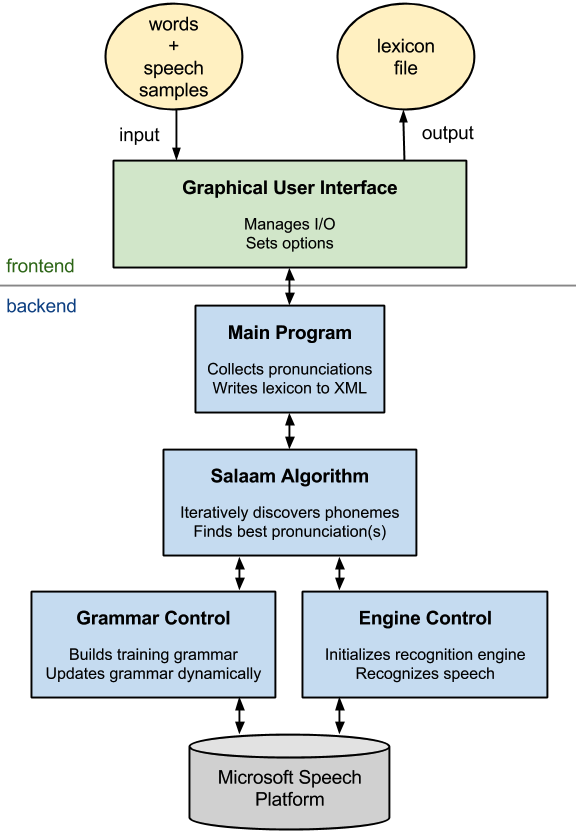
\includegraphics[width=\columnwidth]{../img/SystemOverview-compact.png}
\caption{Overview of the core components of the \textit{lex4all} lexicon-building application.\label{fig:system}}
\end{center}
\end{figure}

Once pronunciations for all terms in the vocabulary have been generated, the application outputs a pronunciation lexicon for the given terms as an XML file conforming to the Pronunciation Lexicon Specification\footnote{http://www.w3.org/TR/pronunciation-lexicon/} (see Figure~\ref{fig:lexicon}). This lexicon can then be directly included in a speech recognition application built using the Microsoft Speech Platform API or a similar toolkit.




%Figure~\ref{fig:lexicon} shows a sample lexicon XML file conforming to the Pronunciation Lexicon Specification \cite{pls}. A lexicon is composed of one \texttt{lexeme} element for each term-sound pairing. In a lexicon intended for speech recognition, each \texttt{lexeme} consists of one \texttt{grapheme} element, representing the term's orthographic form, and one or more \texttt{phoneme} elements, each containing a sequence of phonemes that constitutes an acceptable pronunciation of the term. 


\section{Pronunciation mapping}
\label{sec:backend}

\subsection{Recognition engine}
\label{sec:engine}
%As described above, \textit{lex4all} uses a recognition engine trained for a HRL to map audio in the target LRL to pronunciations (phoneme sequences) in the source HRL. 
%In the current implementation, 
For the HRL recognizer
we use the American English recognition engine 
%developed by Microsoft for server-side recognition of telephone-quality audio, accessed via 
of the Microsoft Speech Platform \cite{mspsdk}. 
%In keeping with the overall objective of the Salaam approach, 
The engine is used as-is, with no modifications to its underlying models. 
We choose the Microsoft Speech Platform for its robustness and ease of use, as well as to maintain comparability with the work of \newcite{Qiao10} and \newcite{Chan12}, who also used Microsoft's server-side American English recognizer. 
Following these authors, we use an engine designed for server-side recognition of low-quality audio, since we aim to enable the creation of useful applications for LRLs, including those spoken in developing-world communities, and such applications will most likely need to cope with telephone-quality audio or similar (see e.g. \newcite{case4st4d}).



\subsection{Implementation of the Salaam method}
\label{sec:implementation}

Pronunciations (sequences of source-language phonemes) for each term in the target vocabulary are generated using the iterative Salaam algorithm %\cite[Sec.~4.1]{Qiao10}, 
described in Section~\ref{sec:background}. In our implementation, 
%we follow \newcite[p. 2]{Chan12} in taking all sequences returned in a given pass as input for the following pass, and 
%we slightly modify the algorithm's stopping condition to terminate 
we stop iterations
if the top-scoring sequence for a given word has not changed for three consecutive iterations \cite{Chan12}, or 
%-- following \newcite{Qiao10} --  
if the best sequence from the $i^{th}$ pass has a lower score than the best sequence of the ${i - 1}^{th}$ pass (with the ${i - 1}^{th}$ results returned as the best pronunciations) \cite{Qiao10}. In both cases, at least three passes are required. 

%To determine the best pronunciation sequences for a given term from each pass, the results for all training samples of that term are naively combined into a set, and sorted by the confidence score assigned to each pronunciation (phoneme sequence). If a given pronunciation matches more than one sample, the overall score for that sequence in that pass is simply the sum of confidence scores for all samples it was associated with. In future work, it may be worth exploring more intelligent heuristics for ranking the set of sequences (see Section~\ref{sec:future}).

After the iterative training has completed, the $n$-best pronunciation sequences (with $n$ specified by the user -- see Section~\ref{sec:options}) for each term are written to the lexicon, each in a \texttt{phoneme} element corresponding to the \texttt{grapheme} element containing the term's orthographic form (e.g. Figure~\ref{fig:lexicon}).

\subsection{Running time}
\label{sec:runningtime}

A major challenge we faced in engineering a user-friendly application based on the Salaam algorithm 
%\cite{Qiao10} 
was its long running time. 
%By slightly modifying the recognition grammar used, we reduce training time by at least a factor of 10, yet at no cost to the accuracy of the resulting lexicon.
%
As stated in Section~\ref{sec:background}, this algorithm
%described by \newcite{Qiao10} 
depends on a ``super-wildcard'' grammar that allows the recognizer to match each sample of a given term to a ``phrase'' of 0-10 ``words'', each word comprising any possible sequence of 1, 2, or 3 source-language phonemes. Given the 40 phonemes of American English, this gives over 65,000 possibilities for each word, resulting in a huge training grammar and thus a long processing time. For a 25-term vocabulary with 5 training samples per term, we found the process to take approximately 1-2 hours
on a standard modern laptop. 
%This is well beyond the amount of time that a developer will wish to spend creating just one component (the lexicon) of their speech-driven application, especially for a meager 25-term lexicon. 
For development and research, this long training time is a serious disadvantage.
%, especially given the fact that real applications may require even larger vocabularies.

To speed up training, we limit the length of each ``word'' in the grammar to only one phoneme, instead of up to 3, giving e.g. 40 possibilities instead of tens of thousands. 
%Despite the shorter word sequences, this implementation of 
The algorithm can still discover pronunciation sequences of an arbitrary length, since, in each iteration, the phonemes discovered so far are prepended to the super-wildcard grammar, such that phoneme sequence of the first ``word'' in the phrase grows longer with each pass 
\cite
%[p.~4]
{Qiao10}. 
However, the new implementation is an order of magnitude faster: constructing the same 25-term lexicon on the same hardware takes approximately 2-5 \textit{minutes}, i.e. less than 10\% of the previous training time.

To ensure that the new implementation's vastly improved running time does not come at the cost of reduced recognition accuracy, we evaluate and compare word recognition accuracy rates using lexicons built with the old and new implementations. The data we use for this evaluation is a subset of the Yoruba data collected by 
\newcite
%[Sec.~5.1]
{Qiao10}, 
comprising 25 Yoruba terms (words) uttered by 2 speakers (1 male, 1 female), with 5 samples of each term per speaker. 
To determine same-speaker accuracy for each of the two speakers, we perform a leave-one-out evaluation on the five samples recorded per term per speaker. 
%(this amounts to a five-fold evaluation, reserving one sample per term per speaker for testing, and training on the other four). 
Cross-speaker accuracy is evaluated by training the system on all five samples of each term recorded by one speaker, and testing on all five samples from the other speaker.
%Using R\footnote{http://www.r-project.org/} 
We perform a paired two-tailed $t$-test on the results to assess the significance of the differences in accuracy.

\begin{table}[tb]
\begin{center}
\begin{tabularx}{\columnwidth}{p{1mm} p{3mm} l r r r}
\hline
 & & & Old & New & $p$\\
\hline
\noalign{\smallskip}

%\multicolumn{2}{l}{\parbox{3.7cm}{Approx. training time, 25 terms (minutes)}} & 60-120 & 2-5 & \\
%\noalign{\smallskip}
%\hline
%\noalign{\smallskip}

%\multirow{3}{*}{\begin{sideways}Same-speaker\end{sideways}}
%\multicolumn{2}{l}{\textit{Same-speaker results}}\\
& & Female  average & 72.8 & \textbf{73.6} & 0.75 \\
& & Male  average & \textbf{90.4} & \textbf{90.4} & 1.00\\
\multirow{-3}{*}{\begin{sideways} Same-\end{sideways}}& \multirow{-3}{*}{\begin{sideways} speaker \end{sideways}}& Overall average & 81.6 & \textbf{82} & 0.81 \\

\noalign{\smallskip}
\hline
\noalign{\smallskip}

%\multirow{3}{*}{\rotatebox{90}{Cross-speaker}}
%\multicolumn{2}{l}{\textit{Cross-speaker results}} \\
&& Trained on male& \textbf{70.4} & 66.4 & --\\
&& Trained on female & 76.8 & \textbf{77.6} & --\\
\multirow{-3}{*}{\begin{sideways}{ Cross-}\end{sideways}}&\multirow{-3}{*}{\begin{sideways}{ speaker}\end{sideways}}& Average & \textbf{73.6} & 72 & 0.63\\

\noalign{\smallskip}
\hline
\end{tabularx}
\end{center}
\caption{Difference in word recognition accuracy for Yoruba 
%(25~words, 2~speakers, 5~samples per word per speaker) 
using old (slower) and new (faster) implementations, with $p$-values from 
%paired two-tailed 
$t$-tests. Bold values represent highest accuracy. \label{tab:accuracy}}
\end{table}

The results of our evaluation, given in Table~\ref{tab:accuracy}, indicate no statistically significant difference in accuracy between the two implementations 
(all $p$-values are above 0.5 and thus clearly insignificant).  
%by making this simple modification to the wildcard grammar used for pronunciation discovery, we achieve an
As our new, modified implementation of the Salaam algorithm 
is much faster than the original, yet equally accurate,
\textit{lex4all} uses the new implementation by default, although for research purposes we leave users the option of using the original (slower) implementation (see Section~\ref{sec:options}).



%%% OLD (BIG) TABLE
%\begin{table*}[t]
%\begin{center}
%
%\begin{tabular}{lrccrr}
%%{
%%\toprule
% &  & \multicolumn{2}{c}{Word Recognition Accuracy (\%)} & Difference & $p$-value \\
%\cmidrule(rl){3-4}
%& & Old wildcard & New wildcard & &  \\
%\midrule
%\addlinespace
%Same-speaker & Female (avg.) & 72.8 & \textbf{73.6} &+0.8 & 0.75 \\
%(leave-one-out)		& Male (avg.) & \textbf{90.4} & \textbf{90.4} & 0.0 & 1.00 \\
%			& Overall average & 81.6 & \textbf{82} &  +0.4 & 0.81 \\
%\addlinespace
%\addlinespace
%
%%\midrule
%\addlinespace
%Cross-speaker	&Male $\rightarrow$ Female & \textbf{70.4} & 66.4 & -4.0 & \\
%(train $\rightarrow$ test)		& Female $\rightarrow$ male & 76.8 & \textbf{77.6}& +0.8	&  \\
%			&Average & \textbf{73.6} & 72 	&-1.6	& 0.63 \\
%\addlinespace
%%\addlinespace
%\midrule
%%}
%\end{tabular}
%\end{center}
%\caption{Word recognition accuracy using American English recognizer on Yoruba audio (25~words, 2~speakers, 5~samples per word per speaker), with results of paired two-tailed $t$-test for significance.\label{tab:accuracy}}
%\end{table*}



\subsection{Discriminative training}
\label{sec:discrimtrain}
%We implement the iterative discriminative training algorithm of \newcite{Chan12} and offer it as an optional step in the lexicon-building process. 
As explained in Section~\ref{sec:background}, \newcite{Chan12} achieve increased accuracy (gains of up to 5 percentage points) by applying an iterative discriminative training algorithm.
%to the pronunciations discovered by the algorithm of \newcite{Qiao10}.
This algorithm takes as input the set of mapped pronunciations generated using the Salaam algorithm \cite{Qiao10};
in each iteration, it simulates recognition of the training audio samples using these pronunciations, and outputs a ranked list of the pronunciations in the lexicon that best match each sample according to the recognizer. 
Pronunciations that cause ``confusion'' between words in the vocabulary, i.e. pronunciations that the recognizer matches to samples of the wrong word type, are thus identified and removed from the lexicon, and the process is repeated in the next iteration. 
%\newcite[p.~5]{Chan12} report improved accuracy (gains of up to 5 percentage points) with up to 8 iterations.

We implement this accuracy-boosting algorithm in \textit{lex4all}, and apply it by default. 
%However, as \newcite[p.~5]{Chan12} caution that careful selection of the number of iterations is necessary to achieve the highest accuracy,
To enable fine-tuning and experimentation,
we leave users the option to change the number of passes (4 by default) or disable discriminative training entirely, as mentioned in Section~\ref{sec:options}.





\section{User interface}
\label{sec:frontend}

As mentioned above, we aim to make the creation and evaluation of lexicons simple, fast, and above all accessible to users with no expertise in speech or language technologies. Therefore, the application makes use of a simple graphical user interface that allows users to quickly and easily specify input and output file paths, and to control the parameters of the lexicon-building algorithms. 

Figure~\ref{fig:mainform} shows the main interface of the \textit{lex4all} lexicon builder. This window displays the terms the user has specified and the number of audio samples that the user has selected for each word. Another form, accessed via the "Add word" or "Edit" buttons, allows users to add to or edit the vocabulary by simply typing in the desired orthographic form of the word and selecting the audio sample(s) to be used for pronunciation discovery (see Section~\ref{sec:recording} for more details on audio input).


Once the target vocabulary and training audio have been specified, and the additional options have been set if desired, the user clicks the ``Build Lexicon'' button and specifies the desired name and target directory of the lexicon file to be saved, 
and pronunciation discovery begins. 
%In case of errors (e.g. there are terms in the vocabulary for which no audio files have been specified), a message pops up instructing the user on how to correct the error. 
%Once any errors have been resolved, pronunciation discovery begins, and a progress bar appears above the ``Build Lexicon'' button to keep the user informed of the program's status. 
When all pronunciations have been generated, a success message displaying the elapsed training time is displayed, and the user may either proceed to the evaluation module to assess the newly created lexicon (see Section~\ref{sec:evaluation}), or may return to the main interface to build another lexicon. 

\begin{figure}[tb]
\begin{center}
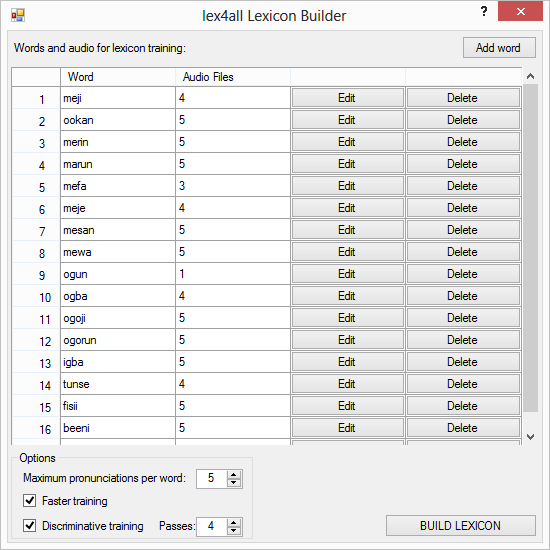
\includegraphics[width=\columnwidth]{../screenshots/LexiconBuilder-Main-Filled-scrolling.PNG}
\caption{Screenshot of the lexicon builder.\label{fig:mainform}}
\end{center}
\end{figure}

\subsection{Audio input and recording}
\label{sec:recording}

%Things to mention (Max, please add to this):
%\begin{itemize}
%\item{NAudio}
%\end{itemize}

%The idea we had in mind was that in addition to uploading existing .wav files it would be interesting to let users record their own audio or ask friends and colleagues to support them. Especially in an international research context such as the one we were developing our tool in that was valuable. 
The GUI allows users to easily browse their file system for pre-recorded audio samples (\texttt{.wav} files) to be used for lexicon training. 
To simplify data collection and enable the development of lexicons even for zero-resource languages, \textit{lex4all} also offers a simple built-in audio recorder to record new speech samples.
%However, as \textit{lex4all} has been designed as a language-independent tool, it should enable the development of applications even in zero-resource languages for which no recorded audio is yet available; to this end, the application includes a built-in audio recorder, to simplify the process of collecting audio samples from native speakers.

%As the backend for the recording feature we use the open-source library NAudio.\footnote{http://naudio.codeplex.com/}
% The package offers classes and methods for a variety of audio-related tasks. Essential for us was the access to I/O and volume control, in particular the classes \textit{waveIn}, \textit{waveFileWriter} and \textit{mixerLine}. 
The recorder, 
built using the open-source library NAudio,\footnote{http://naudio.codeplex.com/}
takes the user's default audio input device as its data source and records one channel with a sampling rate of 8 kHz, since
%We use this low sampling rate because 
the recognition engine we employ is designed for low-quality audio (see Section~\ref{sec:engine}).
%This fixed setup is due to the fact that we simply prefer low-quality audio because the MS speech recognition aims better results with it.  

%A simple GUI form allows users to record audio samples for a given word that has been or is being added to the lexicon vocabulary. Recorded files can be used immediately for lexicon training and/or saved for future use, and can be combined with pre-recorded audio files for training. 

%Although \textit{lex4all}'s audio recording functionality is simple, ...

%Basically two events are handling the input flow. The first one is triggered whenever the record button is not pressed, i.e. whenever the input is not redirected from source to file. Instead it is forwarded to a sample aggregator which stores the maximum volume level of a fixed amount of samples and transmits this value after the amount of samples is reached. The volume level is then displayed on an integrated bar. The reason for the usage of the aggregator is that it would simply overflow the GUI, namely 8000 samples per second. Now we only show 80 samples each second.

%When sound is recorded the data flows straight from the source to a temporary file. Temporary because it is up to the user if we wants to store the file permanently or override it with a subsequent recording. If the first option was chosen the file is also added to the corresponding word as training audio.

\subsection{Additional options}
\label{sec:options}

The lower left corner of the screenshot in Figure~\ref{fig:mainform} shows 
%the parameters and additional options which users can easily modify, if they so choose. 
optional controls for quick and easy fine-tuning of the lexicon-building process (the default settings are pictured).

First of all, users
can specify the maximum number of pronunciations (\texttt{phoneme} elements) per word that the lexicon may contain. According to 
\newcite
%[Sec.~5.2.3]
{Qiao10} and 
\newcite
%[Sec.~4.2.1]
{Chan12}, 
more pronunciations per word in the lexicon may 
%make the lexicon more robust and thus 
improve recognition accuracy.
Secondly, users may train the lexicon using our modified, much faster implementation of the Salaam algorithm or the original implementation 
%more closely 
following \newcite{Qiao10}, as explained in Section~\ref{sec:backend}.
Finally, as mentioned in Section~\ref{sec:discrimtrain}, users may choose whether or not discriminative training 
%algorithm of \newcite{Chan12} 
is applied, and if so, how many passes are run.

%We offer access to these options via the GUI so that users can quickly and easily fine-tune the lexicon-building process
%, possibly to experiment with different settings to achieve the highest possible recognition accuracy. 

%In conjunction with the application's evaluation module (see Section~\ref{sec:evaluation}), this expedites further research into language-independent small-vocabulary recognition. However, users who do not wish to change the default settings (shown in Figure~\ref{fig:mainform}) may simply ignore these controls.



\section{Evaluation module for research}
\label{sec:evaluation}

In addition to its primary utility as a lexicon-building tool, \textit{lex4all} is also a valuable research aide thanks to an evaluation module that allows users to quickly and easily evaluate the lexicons they have created. The evaluation tool allows users to browse their file system for an XML lexicon file that they wish to evaluate; this may be a lexicon created using \textit{lex4all}, or any other lexicon in the same format. 
%The application reads this lexicon and automatically populates a list of its words (\texttt{grapheme} elements), displaying them in a window similar to that of Figure~\ref{fig:mainform}; users may remove words from the evaluation set, but may not add any words that are not included in the lexicon file. 
As in the main interface, users then select one or more audio samples (\texttt{.wav} files) for each term they wish to evaluate.
%, which will be used for testing. 
%At the click of a button, the 
The system then attempts to recognize each sample using the given lexicon, and reports the counts and percentages
of correct, incorrect, and failed recognitions.
%of samples correctly and incorrectly recognized, and the number (if any) that could not be recognized. 
Users may optionally save this report, along with a confusion matrix of word types, as a comma-separated values (\texttt{.csv}) file.
%, which can be easily imported into standard spreadsheet or statistical analysis software for analysis of the results. 

The evaluation module thus allows users to quickly and easily assess different configurations of the lexicon-building tool, by simply changing the settings using the GUI (see Section~\ref{sec:options}) and evaluating the resulting lexicons. Furthermore, as the application's source code is freely available and modifiable, researchers may even replace entire modules of the system 
(e.g. use a 
%recognition engine for a different source language, or a different 
different recognition engine or 
pronunciation-discovery algorithm), and use the evaluation module to quickly assess the results. 
Therefore, \textit{lex4all} facilitates not only application development but also further research into small-vocabulary speech recognition using mapped pronunciation lexicons.
%into language-independent small-vocabulary speech recognition. 

\section{Conclusion and future work}
\label{sec:future}

We have presented \textit{lex4all}, an open-source application that enables the rapid automatic creation of pronunciation lexicons in any (low-resource) language, using an out-of-the-box commercial recognizer \cite{mspsdk} for a high-resource language (English) and the Salaam method for cross-language pronunciation mapping \cite{Qiao10,Chan12}. The application thus makes small-vocabulary speech recognition interfaces feasible in any language, since the algorithm requires only minutes of training audio; given the built-in audio recorder, lexicons can be constructed even for zero-resource languages. 
%TODO  draw more focus to evaluation tool?
Furthermore, \textit{lex4all}'s flexible and open design and easy-to-use evaluation module
%We hope that this tool will help developers create speech-driven applications in LRLs, as well as facilitate 
make it a valuable tool for
research in language-independent small-vocabulary recognition.

%Future directions for the development of \textit{lex4all} include the addition of more back-end options to give users even greater control over the lexicon-building process. One logical next step would be
In future work, we plan 
to expand the selection of source-language recognizers; at the moment, \textit{lex4all} only offers American English as the source language, but any of the 20+ other HRLs supported by the Microsoft Speech Platform could theoretically be used, and it would be interesting to investigate different pairings of source and target languages. Another future goal is to improve and extend the functionality of the audio-recording tool (see Section~\ref{sec:recording}), 
%by giving users greater control over e.g. the sampling rate for recordings, and/or by making the tool more user-friendly with e.g. instant playback of recorded audio. 
to make it more flexible and user-friendly.
Finally, as a complement to the application, it would be beneficial to 
create a central online data repository where users can 
%offer users the option to share 
upload the lexicons they have built and the speech samples they have recorded. %by uploading this data to a central online repository. 
Over time, this could become a valuable collection of data for LRLs, enabling developers and researchers to share and re-use data among languages or language families.

% future work on the recording function
%It would be advantageous to display the volume while recording which is at the moment not possible because data is redirected either way. Unfortunately we had issues when doing both simultaneously which resulted in disturbances in the recorded audio.
%A major advantage would it be to play back what has been recorded, so the user does not have to save the file first in order to check its quality and content.

%\section*{Acknowledgments}
%
%The acknowledgments should go immediately before the references.  Do
%not number the acknowledgments section. Do not include this section
%when submitting your paper for review.

% include your own bib file like this:
%\bibliographystyle{acl}
%\bibliography{acl2014}
\bibliographystyle{acl}
\bibliography{lex4all.bib}


\end{document}
